% !TeX root = future.tex
% !TeX encoding = UTF-8
% !TeX spellcheck = en_US

%\documentclass[14pt]{beamer}
\documentclass[aspectratio=169]{beamer} % Other possible values are: 1610, 149, 54, 43 and 32. By default, it is to 128mm by 96mm(4:3)

\usepackage[utf8]{inputenc}
\usepackage[T1]{fontenc}
\usepackage{graphicx}
\usefonttheme{serif}

% no navigation symbols
\setbeamertemplate{navigation symbols}{}

% Text positioning
\usepackage[absolute,overlay]{textpos}

% https://hartwork.org/beamer-theme-matrix/
\definecolor{bulletcolor}{RGB}{0,0,0} % RGB model is defined with values between 0 and 255
\setbeamercolor{local structure}{fg=bulletcolor}
\setbeamertemplate{itemize items}[circle]

% make the hyperlinks blue
\usepackage{hyperref}
\hypersetup{colorlinks=true,urlcolor=blue}

\usepackage{physics}

% Table of Contents at Section start
\AtBeginSection[]
{
	\begin{frame}
		\frametitle{\bfseries\Huge\textcolor{black}{.}}
		\tableofcontents[currentsection]
	\end{frame}
}

\begin{document}

\usebackgroundtemplate{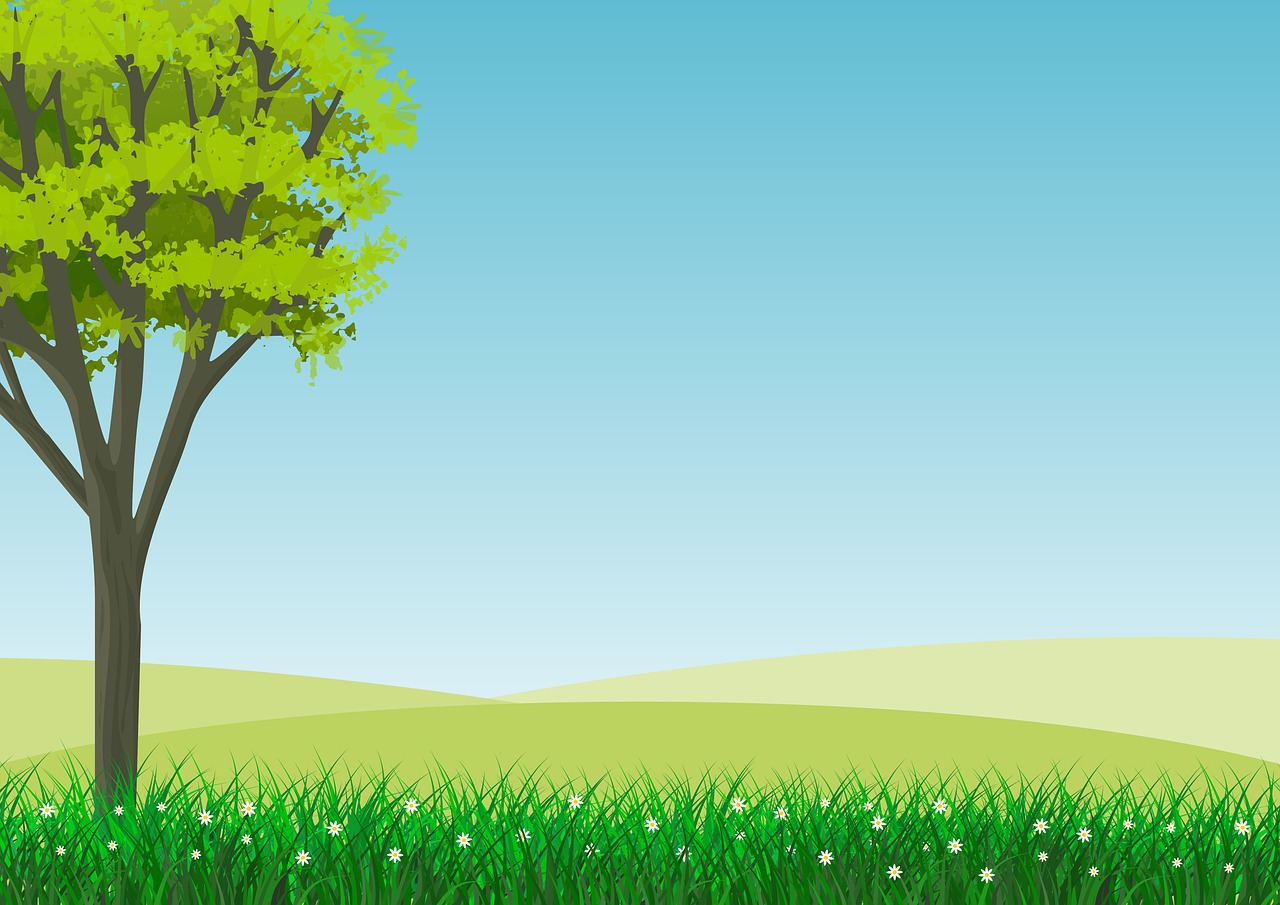
\includegraphics[width=\paperwidth]{../images/tree-5939865_1280.jpg}}
\section{Introduction}
%\note{Image \href{https://pixabay.com/users/aalmeidah-4277022}{aalmeidah from Pixabay}}

\usebackgroundtemplate{
\includegraphics[width=\paperwidth]{../images/field-1728099.jpg}}
\begin{frame}{}
	\setlength{\TPHorizModule}{\textwidth}
	\setlength{\TPVertModule}{\textwidth}
	% Slide title in upper left
	\begin{textblock}{0.74}(0.05,0.05)
		\bfseries\large\normalcolor{introduction}
	\end{textblock}
	% main body bullet points
	\begin{itemize}
		\item A bit of math.
		\item Some of the major players.
	\end{itemize}
\end{frame}
%\note{This is a note.}

% concepts
\begin{frame}
	\frametitle{Vectors and Matrices}
    Vectors are ``columns''
\end{frame}
%\note{This is a note.}

%
\begin{frame}
    \frametitle{Qubits}
    \begin{itemize}
    \item Spin
    \item Trapped Atoms and Ions
    \item Photons
    \item Superconducting Circuits\
	\end{itemize}

\end{frame}
\note{This is a note. https://uwaterloo.ca/institute-for-quantum-computing/quantum-101/quantum-information-science-and-technology/what-qubit}

\begin{frame}
	\frametitle{Some Quick Notation}
    \begin{itemize}
	\item The Greek letter Psi \begin{math}\Psi\end{math}
    \item Dirac notation, including ``bra'' \begin{math}\bra{0}\end{math} and ``ket'' \begin{math}\ket{0}\end{math}
	\item You might see Psi in a ``ket'' like so \begin{math}\ket{\Psi}\end{math}
    \end{itemize}

\end{frame}
%\note{This is a note.}

\usebackgroundtemplate{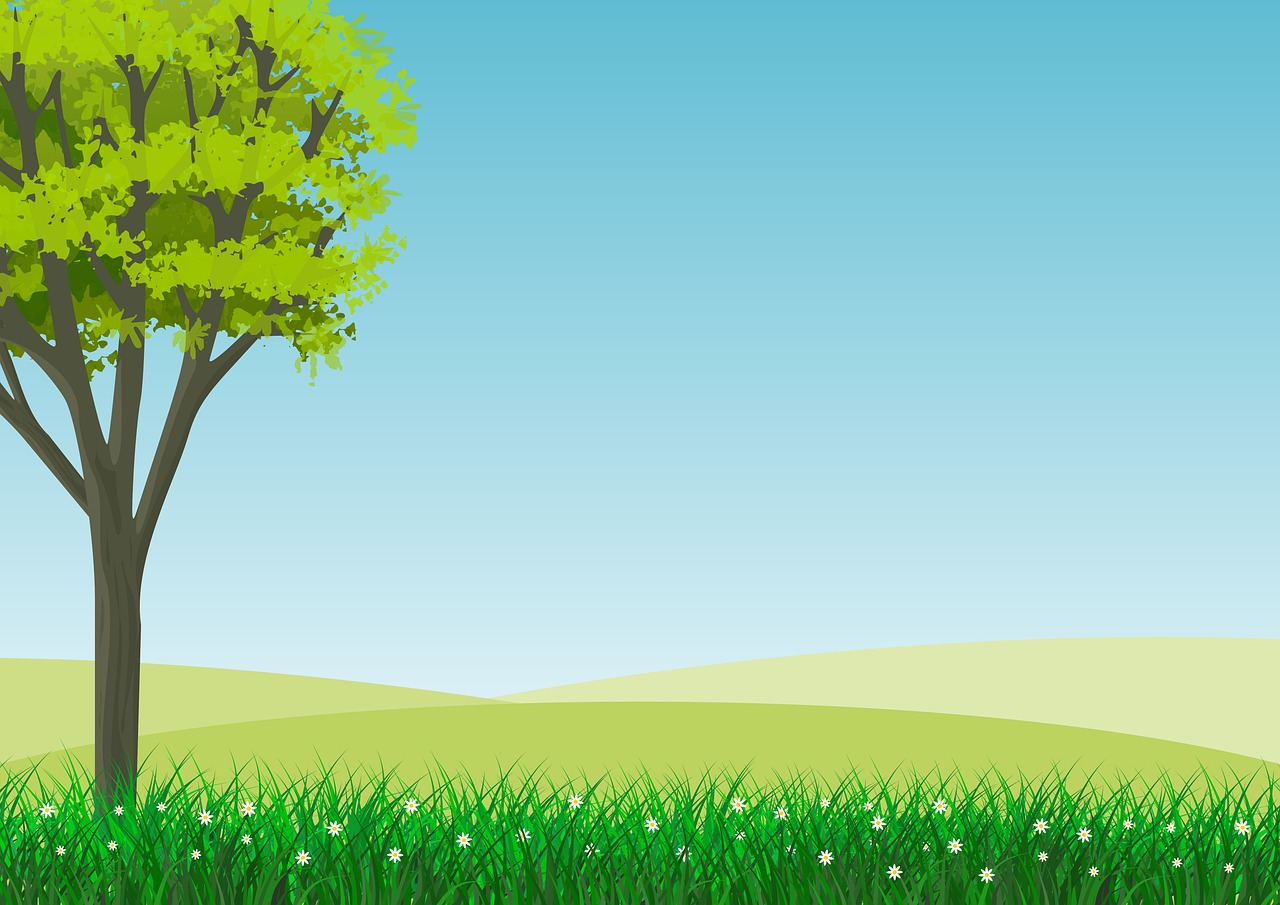
\includegraphics[width=\paperwidth]{../images/tree-5939865_1280.jpg}}
\section{The State of Things}
\usebackgroundtemplate{
\includegraphics[width=\paperwidth]{../images/field-1728099.jpg}}

\begin{frame}
    \frametitle{Quantum Supremacy}
    Lorem ipsum dolor sit amet, consectetur adipisicing elit, sed do eiusmod tempor incididunt ut labore et dolore magna aliqua.
\end{frame}
%\note{This is a note.}

\begin{frame}
\frametitle{Quantum KDCs}
Lorem ipsum dolor sit amet, consectetur adipisicing elit, sed do eiusmod tempor incididunt ut labore et dolore magna aliqua.
\end{frame}
%\note{This is a note.}

\usebackgroundtemplate{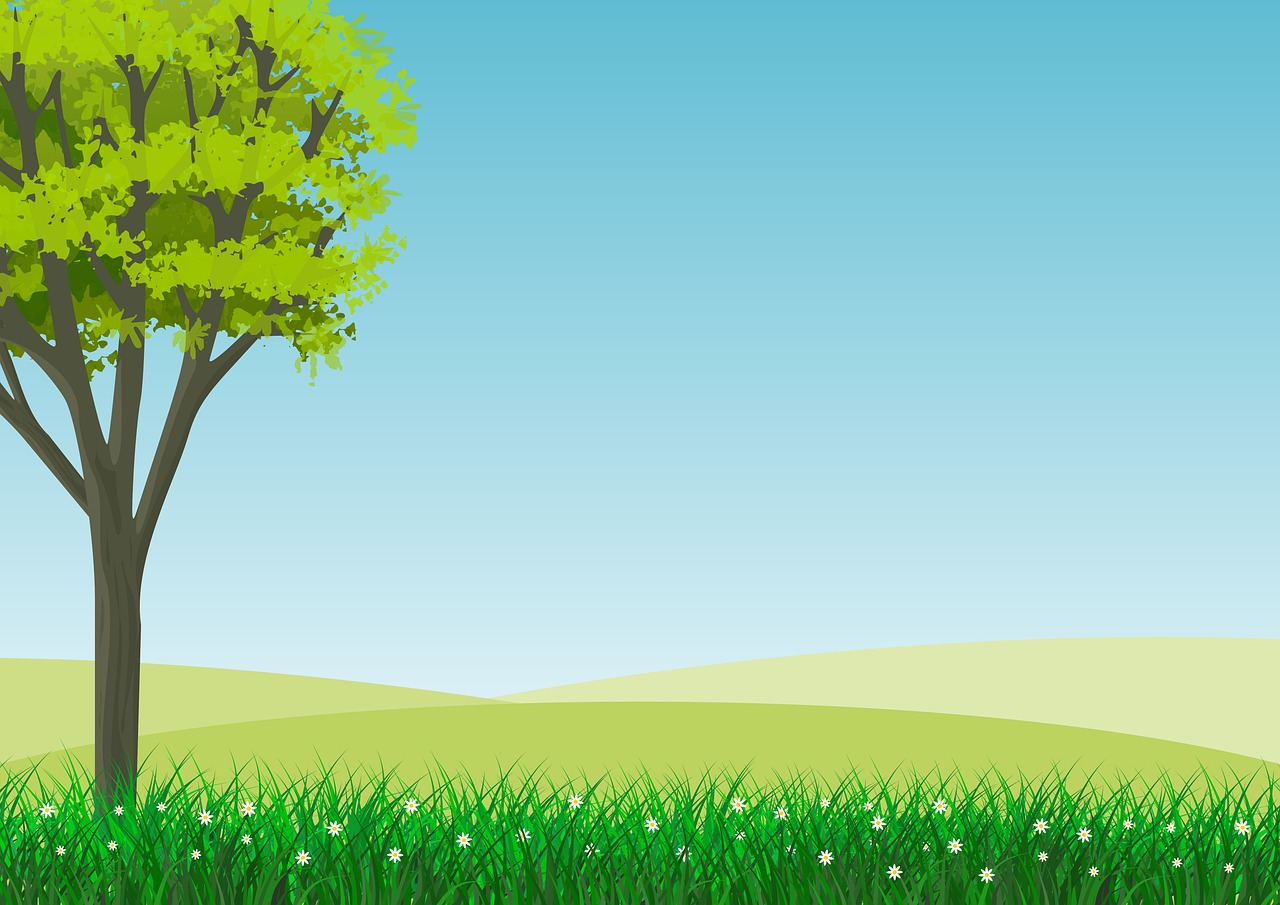
\includegraphics[width=\paperwidth]{../images/tree-5939865_1280.jpg}}
\section{Commercial Efforts}
\usebackgroundtemplate{
\includegraphics[width=\paperwidth]{../images/field-1728099.jpg}}
\begin{frame}{}
    \frametitle{Google}
     \begin{itemize}
         \item \href{https://quantumai.google/cirq/tutorials}{so many free resources!}
         \item \href{https://www.youtube.com/watch?v=16ZfkPRVf2w}{The ``cirq'' module for Python.}
     \end{itemize}
\end{frame}
%\note{This is a note.}

\begin{frame}{}
    \frametitle{DWave}
    \begin{itemize}
        \item What is cirq?
    \end{itemize}
\end{frame}
%\note{This is a note.}

\begin{frame}{}
    \frametitle{IBM}
    \begin{itemize}
        \item \href{https://www.youtube.com/watch?v=o-FyH2A7Ed0}{Souds of IBM Quantum}
    \end{itemize}
\end{frame}
%\note{This is a note.}

\begin{frame}{}
    \frametitle{Amazon}
    \begin{itemize}
        \item amazon-braket-sdk
    \end{itemize}
\end{frame}
%\note{This is a note.}
\end{document}